\documentclass[a4paper,12pt]{exam}

\usepackage[T1]{fontenc}
\usepackage[utf8]{inputenc}
\usepackage[dutch]{babel}
\usepackage{cmbright}

\usepackage{graphicx}
\usepackage[export]{adjustbox}
\usepackage[detect-none, list-final-separator={ en }, per-mode=symbol,
            retain-explicit-plus, output-decimal-marker={,},
            exponent-product={\cdot}, range-phrase={ tot }]{siunitx}
\usepackage[font={small,sf},labelfont={bf},labelsep=endash]{caption}
\usepackage{MnSymbol}

\graphicspath{{figures/}}

\newcommand{\figref}[1]{Figuur~\ref{#1}}
\renewcommand{\eqref}[1]{Vergelijking~\ref{#1}}
\newcommand{\tabref}[1]{Tabel~\ref{#1}}

\newcommand{\rchisq}{\ensuremath{\tilde\chi^2}}

\header{\bfseries Toets data-analyse}{\bfseries NP2}{\bfseries Versie 2}
\footer{}{}{\bfseries\iflastpage{Einde $\blacksquare$}{Lees verder $\filledmedtriangleright$}}


\begin{document}
\suppressfloats[t]
\begin{questions}
  \uplevel{Bram wil de versnelling $a$ bepalen van een treintje dat van een helling afrolt. De helling maakt een hoek van \SI{30}{\degree} met de horizon. Hij meet de afstand die het karretje heeft afgelegd op verschillende tijdstippen door middel van een videometing. Het resultaat van de metingen is weergegeven in \tabref{tab:metingen}. De afstanden zijn gemeten met een onzekerheid van \SI{1}{\centi\meter}. De tijden zijn gemeten met een te verwaarlozen onzekerheid.}

  \begin{table}
    \centering
    \caption{Gemeten afstand als functie van de tijd van het treintje.}
    \label{tab:metingen}
    \begin{tabular}{
        l
        l
        % *{9}{S[table-number-alignment=center,
        %        table-figures-integer=2,
        %        table-figures-decimal=1]}
        % S[table-number-alignment=center,
        %   table-figures-integer=3,
        %   table-figures-decimal=1]
        *{10}l
      }
      $t$ & [\si{\second}] & 0,1 & 0,2 & 0,3 & 0,4 & 0,5 & 0,6 & 0,7 & 0,8 & 0,9 & 1,0 \\
      $s$ & [\si{\meter}] & 0,09 & 0,14 & 0,31 & 0,43 & 0,67 & 0,91 & 1,27 & 1,61 & 2,04 & 2,50 \\
    \end{tabular}
  \end{table}

  \uplevel{Bram verwacht het volgende verband:
  \begin{equation}
    s(t) = \frac{1}{2}at^2.
    \label{eq:versnelling}
  \end{equation}
  Met behulp van Origin heeft Bram de meetgegevens uitgezet in een grafiek en gefit aan \eqref{eq:versnelling}. Zie \figref{fig:metingen-fit}.
  }
  \begin{figure}
    \centering
    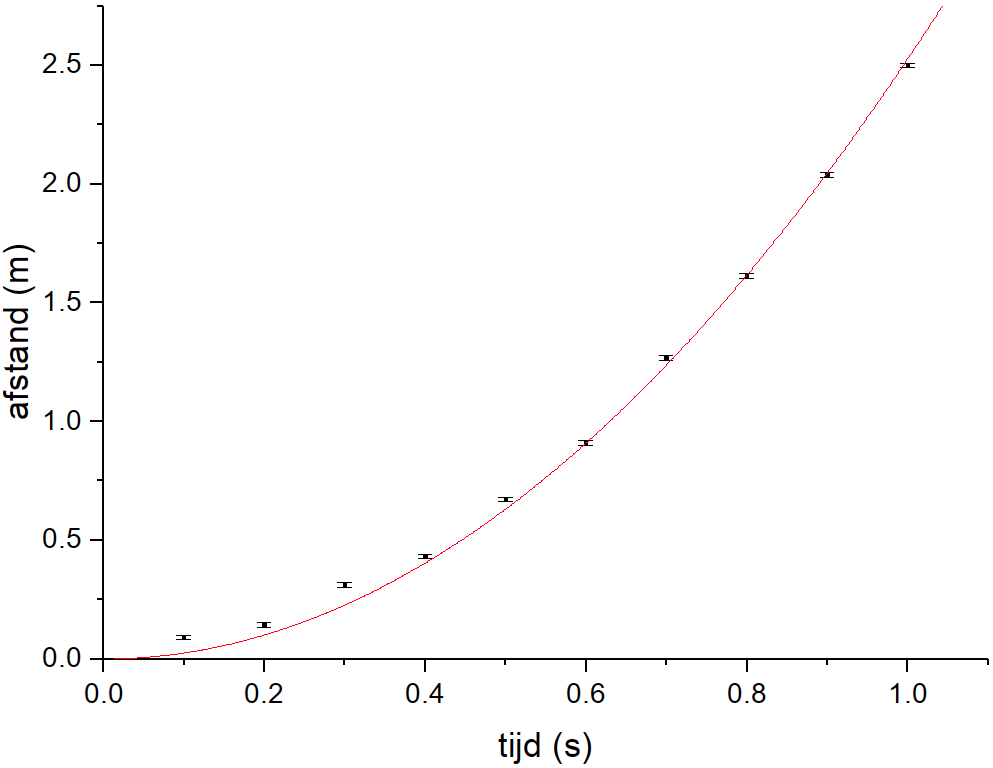
\includegraphics[width=.6\linewidth,valign=t]{fit-helling}
    \hfill
    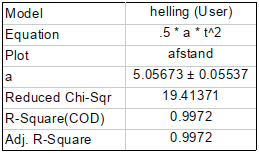
\includegraphics[width=.3\linewidth,valign=t]{fit-parameters-helling}
    \caption{De afstand als functie van de tijd voor een karretje dat van een helling rolt.}
    \label{fig:metingen-fit}
  \end{figure}
  \question Geef de gevonden waarde voor de versnelling $a$, inclusief de onzekerheid, in de juiste notatie.
  \uplevel{Op grond van deze grafiek besluit Bram dat zijn verwachting niet klopt en dat er waarschijnlijk meer aan de hand is.}
  \question Geef daarvoor twee redenen.
  \uplevel{Bram vermoedt dat de afstanden niet goed zijn opgemeten en dat er sprake kan zijn van een systematische fout. Hij besluit nu de data te fitten aan het volgende verband:
  \begin{equation}
    s(t) = s_0 + \frac{1}{2}at^2,
    \label{eq:helling-offset}
  \end{equation}
  met $s_0$ de systematische fout in de afstand $s$. De resultaten staan in \figref{fig:metingen-fit-offset}.}
  \begin{figure}
    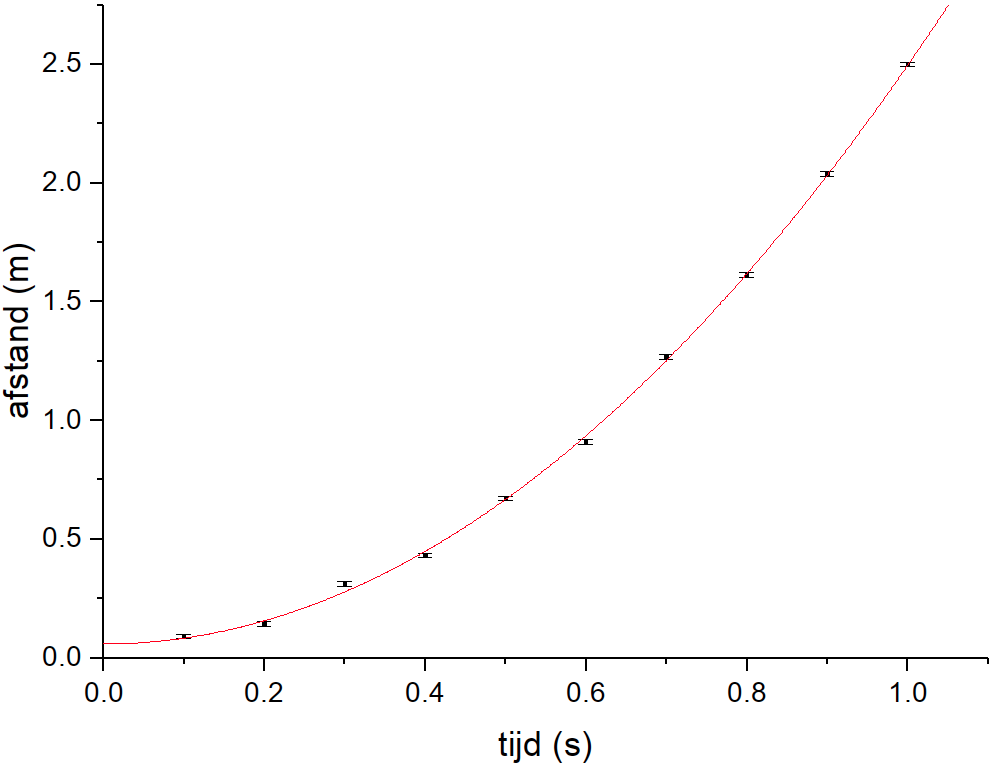
\includegraphics[width=.6\linewidth,valign=t]{fit-helling-offset}
    \hfill
    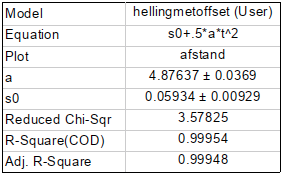
\includegraphics[width=.3\linewidth,valign=t]{fit-parameters-helling-offset}
    \caption{De afstand als functie van de tijd voor een karretje dat van een helling rolt, met systematische fout.}
    \label{fig:metingen-fit-offset}
  \end{figure}
  \uplevel{Bram is nog steeds niet erg tevreden over de fit. De fit ziet er op zich goed uit, maar hij maakt zich zorgen over zijn metingen bij een tijd van \SI{0,3}{\second}. Hij denkt dat hij die meting verkeerd heeft opgeschreven.}
  % \question Bereken de trillingstijd die ze theoretisch zou verwachten bij een lengte van \SI{40}{\centi\meter}. Negeer daarbij de onzekerheid.
  \question Aangenomen dat \eqref{eq:helling-offset} inderdaad geldig is, bereken dan de kans op een meting bij \SI{0,3}{\second} die minstens zo hoog is als de waarde die Bram heeft gevonden. Maak gebruik van Appendix B in Taylor.
  \uplevel{Bram besluit het meetpunt te verwijderen en de fit opnieuw te doen. Hij vindt nu een \rchisq-waarde van \num{0.8}.}
  \question Bereken de bijbehorende $p$-waarde en leg uit wat de betekenis is van een $p$-waarde. Maak gebruik van Appendix D in Taylor.
\end{questions}
\textbf{\rule{5em}{1pt}}
\end{document}
